Come precedentemente specificato sono state estrapolate le entità principali intorno alle quali sviluppare la progettazione. Ciò è stato possibile grazie ad un'approfondita analisi del flusso aziendale, derivato direttamente dall'analisi delle azioni e dei processi interni.\newline
Il risultato è dato dalle cinque seguenti entità fondamentali: \newline

\noindent\makebox[\textwidth]{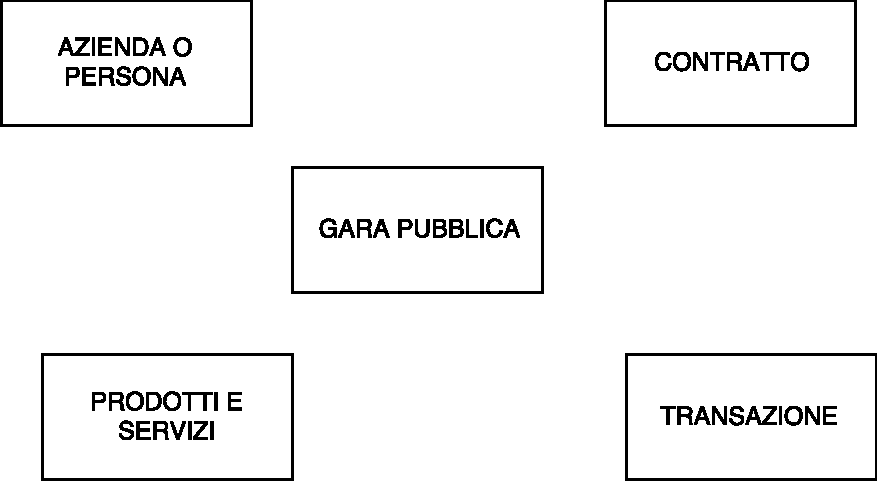
\includegraphics[width=\textwidth-5cm]{./immagini/entita_fondamentali.pdf}}

RICHIESTA SUL MEPA: il blocco rappresenta gli strumenti che le pubbliche amministrazioni utilizzano per  l'interfacciamento con la nostra azienda. In questo caso si parla di gare pubbliche oppure richieste di trattativa dirette. 
PA, AZIENDA O PERSONA: è il macrogruppo comprensivo delle persone giuridiche che hanno rapporti commerciali con la nostra azienda, tra questi ci sono i fornitori e i clienti, sia privati e pubbliche amministrazioni.
PRODOTTO O SERVIZIO: comprende tutti i prodotti vendibili o acquistabili dall'azienda disponibili dai fornitori e i servizi disponibili.
FATTURA: è l'entità fondamentale che interviene in tutte le operazioni sia per l'acquisto che per la vendita di prodotti e/o servizi.

% Gli Oggetti di propriet� del personaggio rappresentano una entit� molto importante, essi possono appartenere anche a un NPC

% \begin{figure}[H]
% \centering
% 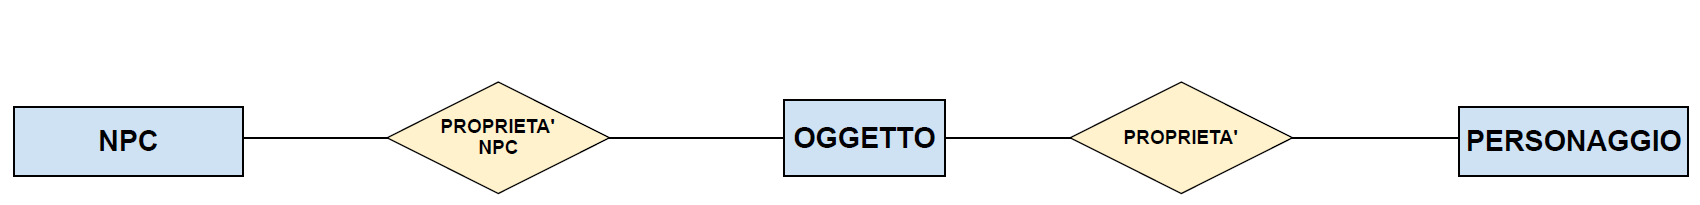
\includegraphics[width=0.7\linewidth]{./immagini/oggettotriplo.png}
% \end{figure}


% All'interno del gioco il personaggio interagisce con altri personaggi ed NPC come descritto nello schema dei processi interni,
% sappiamo che le interazioni di combattimento sono gestite dal Programma e non interessano la Base di Dati, tuttavia una interazione fondamentale �
% la Transazione, in quanto ogni personaggio pu\`{o} vendere oggetti ad un altro o ad un NPC e risulta necessario tenere traccia di queste TRANSAZIONI
%
% I personaggi Intraprendono e completano MISSIONI necessarie all'avanzamento nel gioco
%
% \begin{figure}[H]
% \centering
% 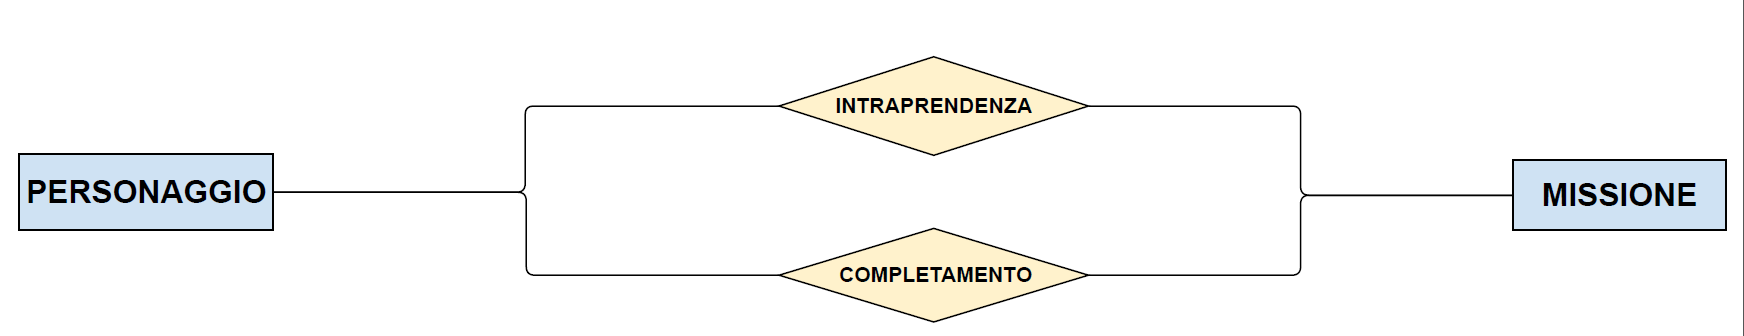
\includegraphics[width=0.7\linewidth]{./immagini/persomiss.png}
% \end{figure}
%
%
% Essi possono inoltre apprendere delle abilit� da degli NPC che le insegnano in cambio di denaro
%
% \begin{figure}[H]
% \centering
% 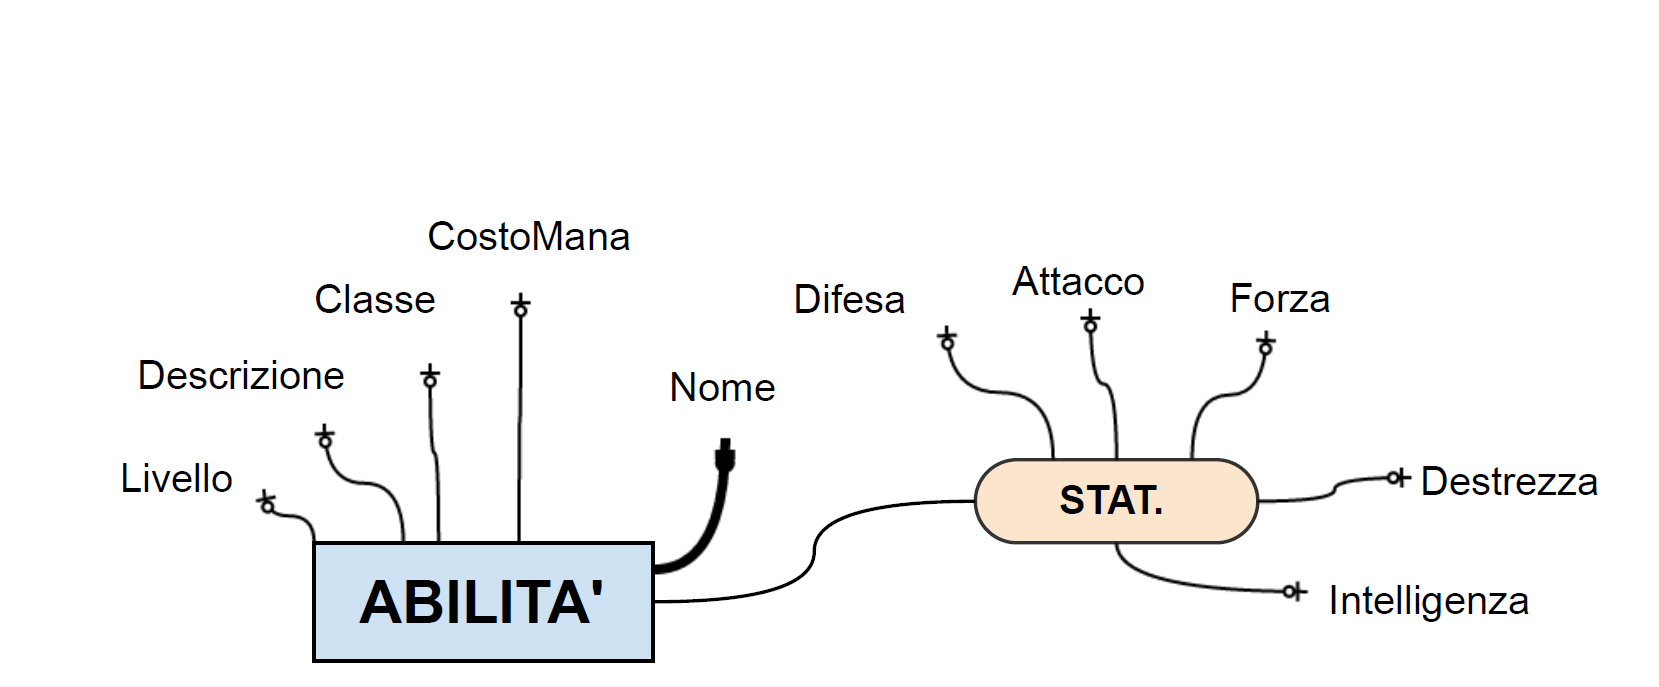
\includegraphics[width=0.7\linewidth]{./immagini/ABILITADEF.png}
% \end{figure}
%
% All'esterno del gioco vero e proprio sappiamo che ci� che accade � principalmente la creazione di personaggi dell'utente e l'acquisto di prodotti dallo store
%
% \begin{figure}[H]
% \centering
% 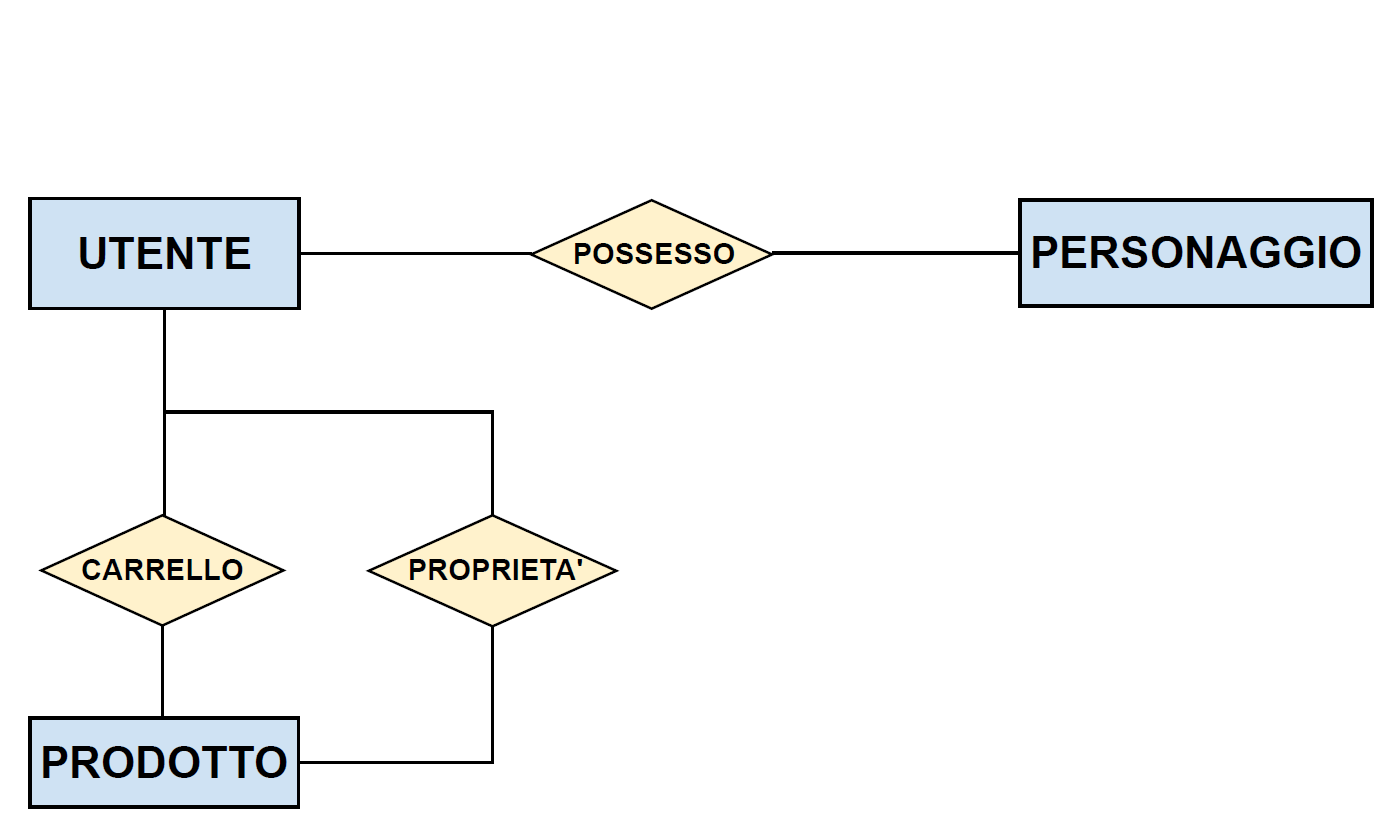
\includegraphics[width=0.7\linewidth]{./immagini/utente.png}
% \end{figure}

\newpage
